\documentclass[./../../paper.tex]{subfiles}
\graphicspath{{\subfix{./../../figures/}}}

\begin{document}

\section{Determine the Evolutionary Algorithm Configurations}

\subsection{Experimental Setup}
\label{sec:exp1}
As explained in \autoref{sec:evolutionary}, there are many possible configurations for an evolutionary algorithm. Therefore, we test combinations of all mentioned configurations for each phase of our evolutionary algorithm.

The combinatory set of all phase options contains \attention{144} elements. To avoid confusion, we refer to each unique phase combination as a configuration. We choose to run each configuration for \attention{50} evolution cycles. For all configurations we use the same set of \attention{5} factual \glspl{instance}, which are randomly sampled from the validation set. We decide to return \attention{500} survivors at the end of each run for every factual case. The initiation phase samples \attention{1000} initial individuals for the population \optional{EXCEPT FittestInitiator, REASON}. Within each cycle, we generate \attention{2000} new offsprings. And choose to add \attention{500} individuals to the population\attention{Revise in code and text}. We keep the mutation rate uniform. Hence, we each delete, insert, change and transpose approximately \attention{20\%} mutation phase. The remaining \attention{20\%} we do not apply any change. We apply each edit-type by a constant edit-rate of \attention{10\%} of the sequence length.

After retrieving the results, we fit a linear mixed-effects model to determine the importance of each configuration. Here, we use the resulting viability as a dependent variable and each phase as independent variable. We adjust the model according to their configuration, as we retrieve \attention{50} samples per configuration. If a phase-type strongly affects the dependent variable and the resulting change is deemed significant, we can draw conclusions about the full configuration. Furthermore, preliminary results showed that many of the configurations have a zero feasibility. Hence, we also incorporate the insights gained from using feasibility as a dependent variable.

\subsection{Results}

% TODO: Change plots to matplotlib plots
\begin{figure}
    \centering
    \begin{subfigure}[c]{0.99\textwidth}
        \centering
        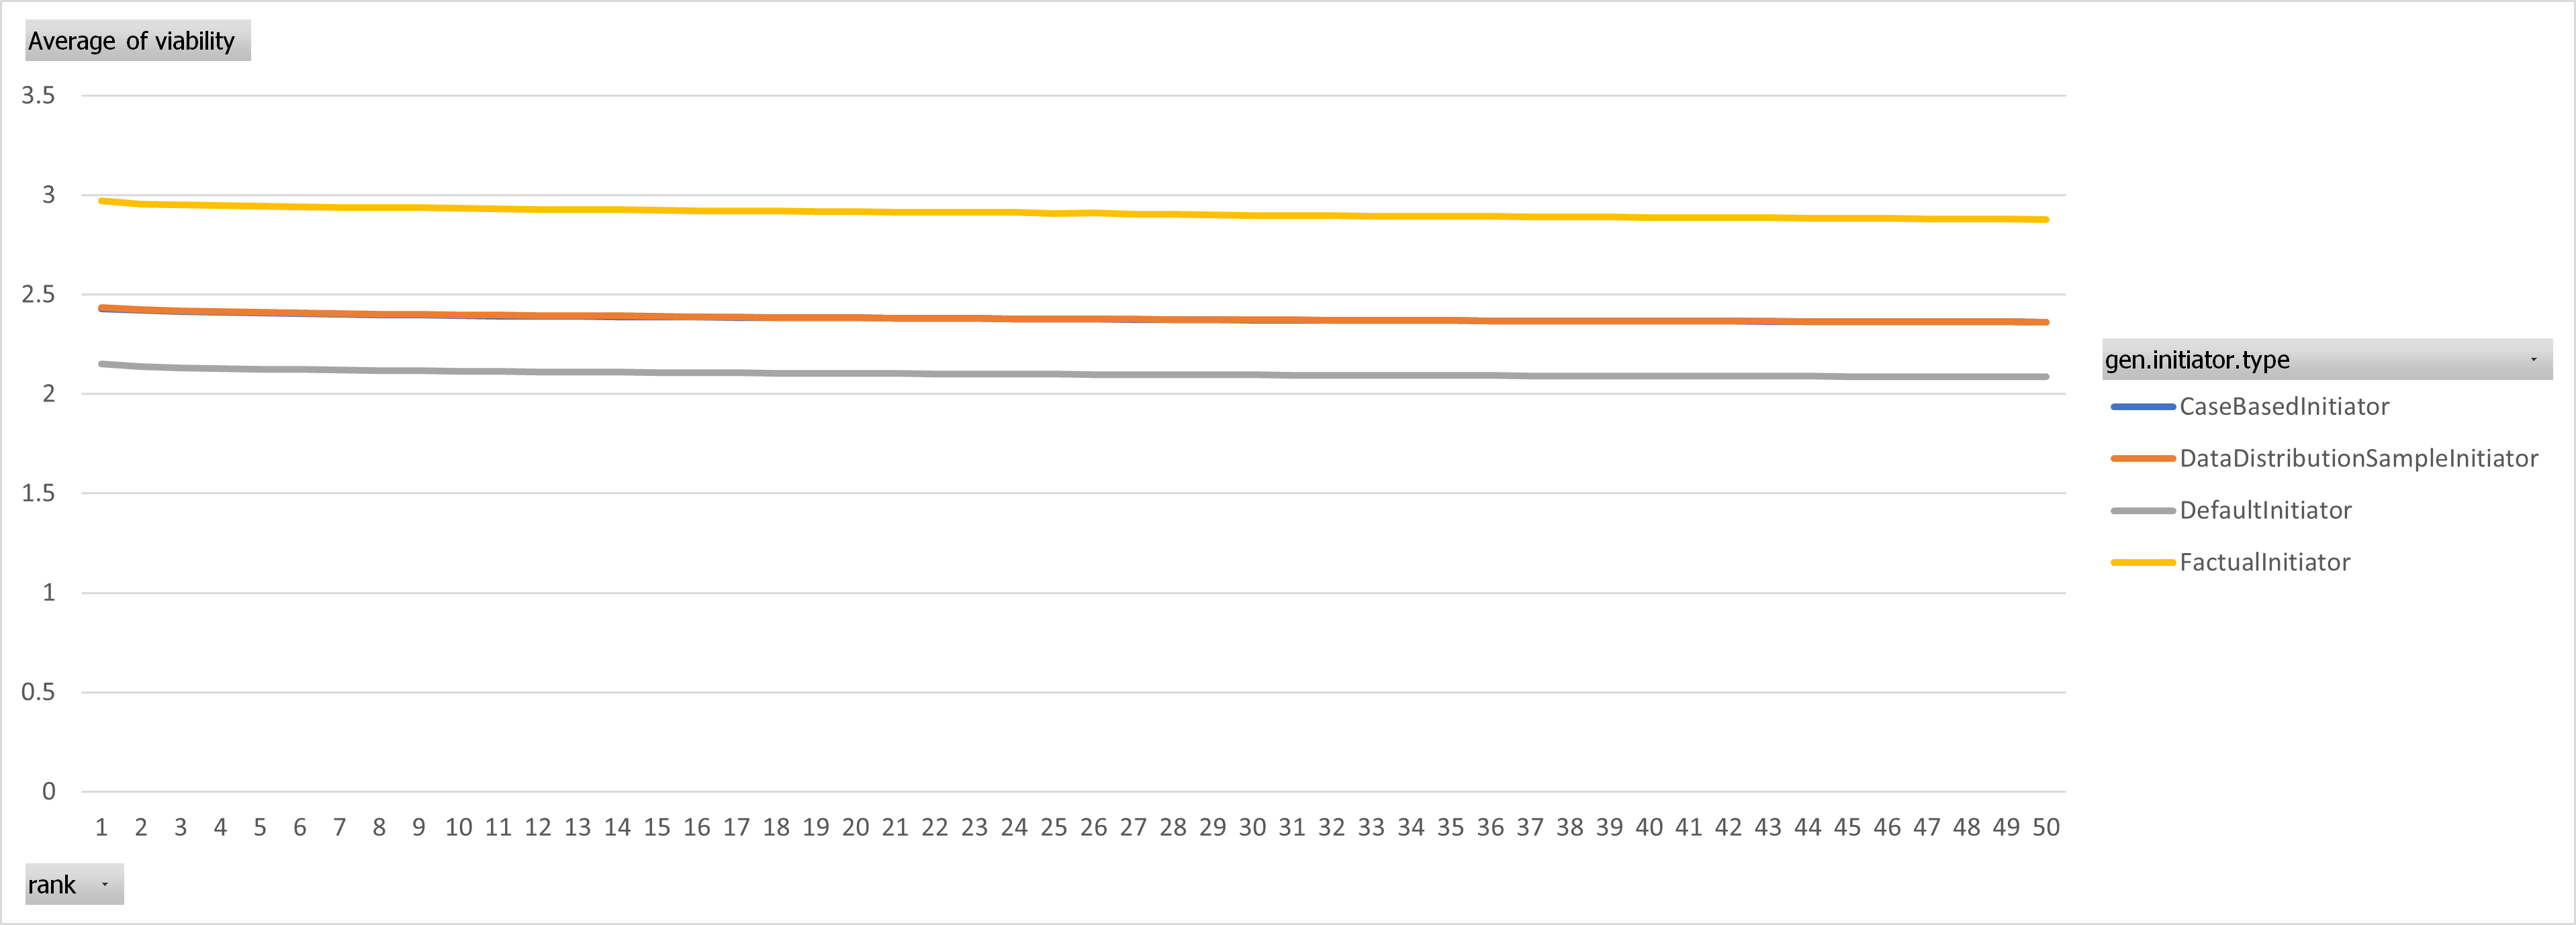
\includegraphics[width=\textwidth]{figures/plots/average_viability.png}
        \caption{This figure shows the average viability of the 50 best counterfactuals for each configuration. The x-axis shows their respective rank. OUTDATED}
        \label{fig:average_viability}
    \end{subfigure}
    \begin{subfigure}[c]{0.99\textwidth}
        \centering
        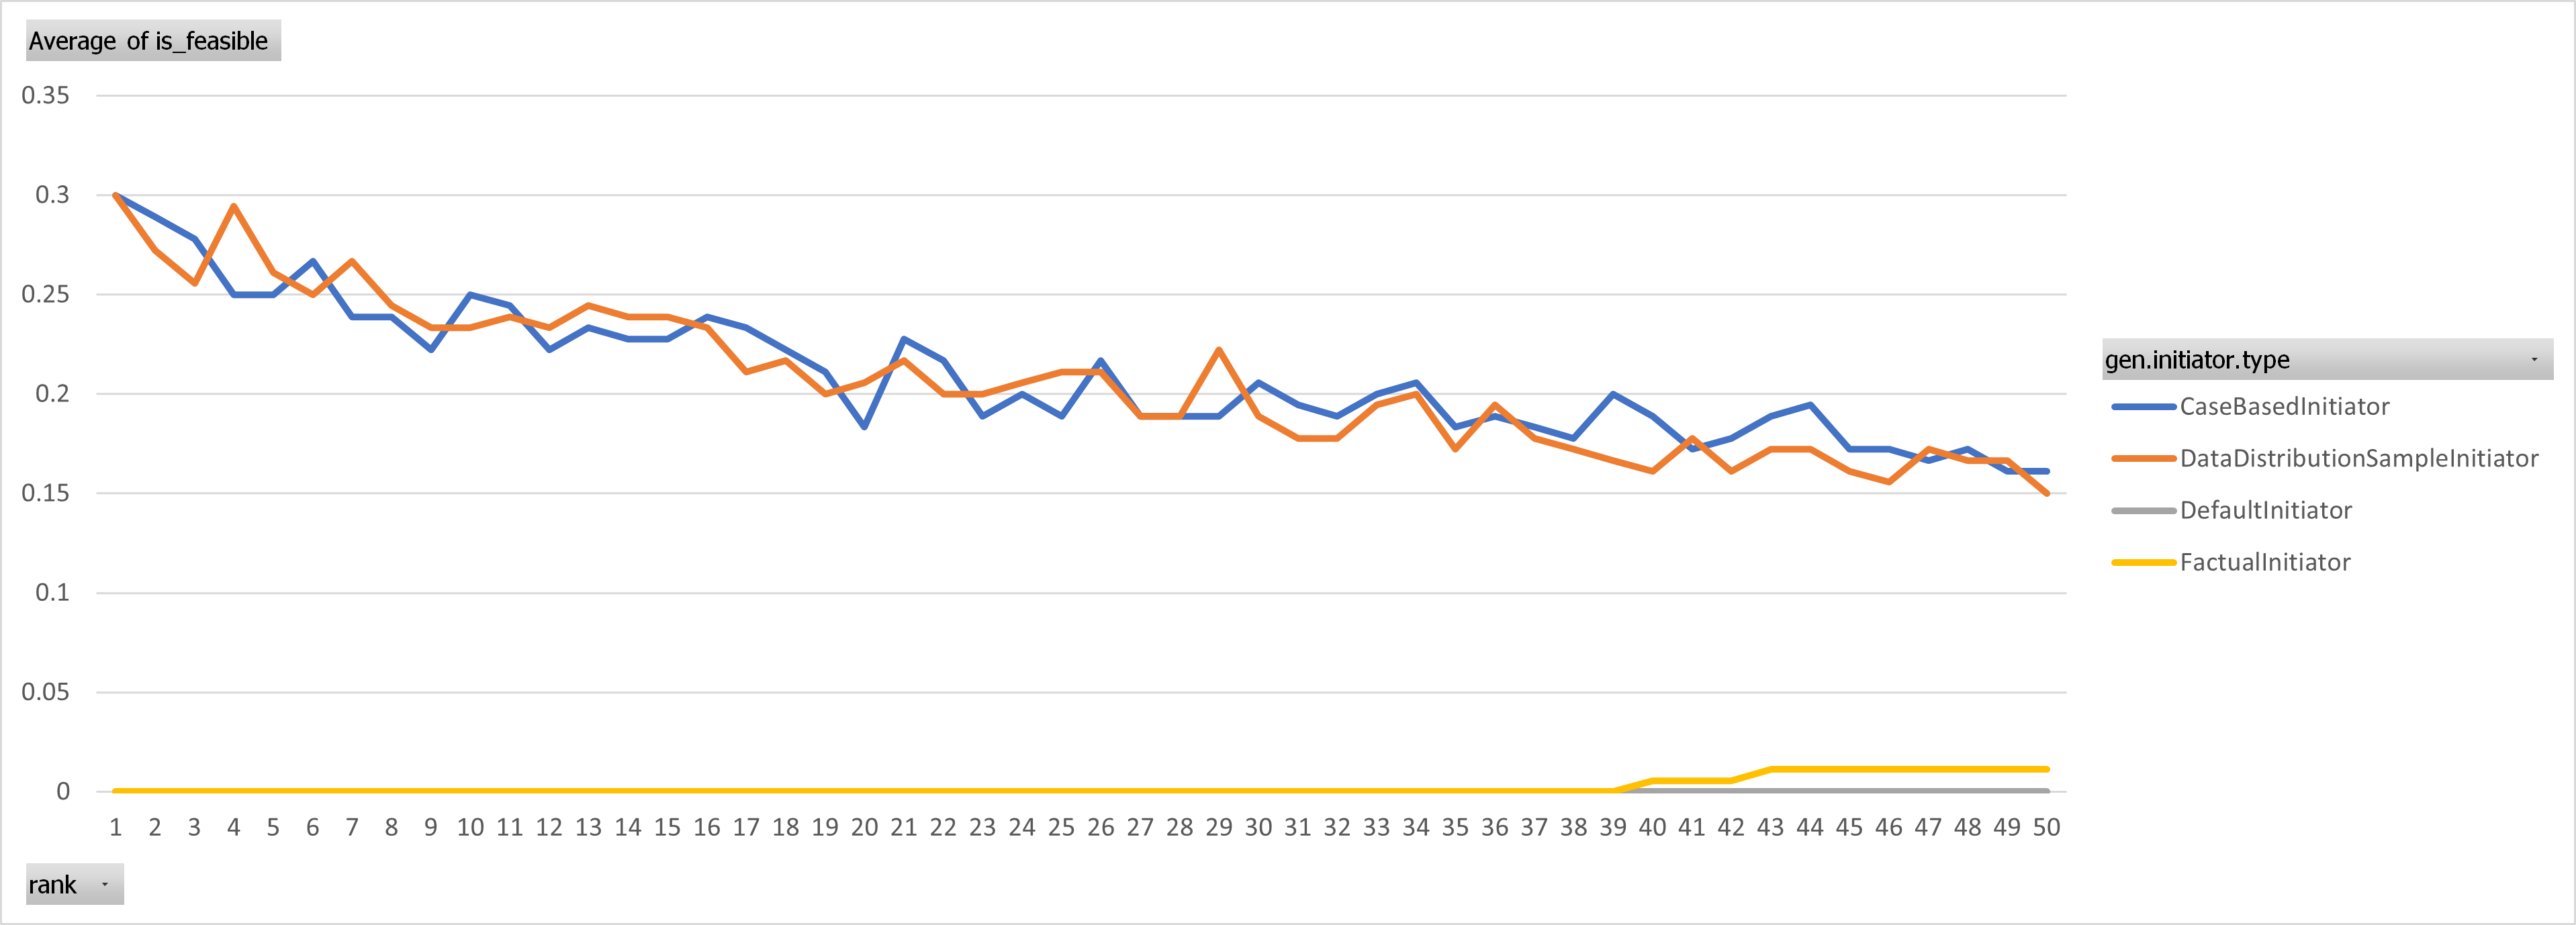
\includegraphics[width=\textwidth]{figures/plots/average_feasibility.png}
        \caption{This figure shows the average feasibility of the 50 best counterfactuals for each configuration. The x-axis shows their respective rank. OUTDATED}
        \label{fig:average_feasibility}
    \end{subfigure}
\end{figure}

\noindent \autoref{fig:average_feasibility} shows for the \attention{DDS} initiator that the fraction of non-zero probability counterfactuals is \attention{20.9\%} and \attention{20.7\%} respectively.  It does not surprise, that the \attention{DI} fails to generate any feasible counterfactual across all configurations.


\begin{table}[htbp]
    \caption{Table shows the result of the linear mixed model. It uses viability as dependent variable and evolutionary operators as independent categorical variable. The model is adjusted for general differences in combinations. The coefficient explains the effect of the model, while P explains the statistical significance. Only significant values are considerable effects.}
    \label{tbl:configs_viability}
    \begin{tabular}{llll}
                                                     & Coef.  & Std.Err. & p-value \\
        Intercept                                    & 2.490  & 0.017    & 0.000   \\
        initiator[T.DataDistributionSampleInitiator] & -0.025 & 0.015    & 0.097   \\
        initiator[T.DefaultInitiator]                & -0.242 & 0.015    & 0.000   \\
        initiator[T.FactualInitiator]                & 0.494  & 0.015    & 0.000   \\
        selector[T.RouletteWheelSelector]            & -0.080 & 0.013    & 0.000   \\
        selector[T.TournamentSelector]               & -0.048 & 0.013    & 0.000   \\
        mutator[T.DefaultMutator]                    & -0.024 & 0.011    & 0.024   \\
        recombiner[T.FittestIndividualRecombiner]    & 0.040  & 0.011    & 0.000   \\
        crosser[T.TwoPointCrosser]                   & 0.003  & 0.013    & 0.833   \\
        crosser[T.UniformCrosser]                    & -0.027 & 0.013    & 0.039   \\
        Configuration Set Var                        & 0.004  & 0.006    &         \\
    \end{tabular}
\end{table}

In terms of viability \autoref{tbl:configs_viability} the overall mean between all configurations is \attention{2.49}. We see that the factual initiator is clearly superior. However, the results for using the factual itself are nearly identical. In terms of the selection operators, we see a reduction of viability using either the \attention{RouletteWheelSelector or TournamentSelector}. Meaning, \attention{the Elitism-Selector} yields better results when it comes to viability. The \attention{DefaultMutator} also reduces the viability. In other words, we achieve better results with the \attention{DataDistributionMutator}. The best recombination approach is the \attention{FittestIndividualRecombiner}. If we had to choose a crossing method, the \attention{TwoPointCrosser} slightly edges out the \attention{OnePointCrosser}. However, this effect is not significant. However, we see, that the \attention{UniformCrosser} reduces viability and it is significant. The effect of each configuration set is comparable with the effect of using the \attention{TwoPointCrosser}. Hence, the composition of configurations plays a comparatively minor role.
% If we consider the ranks of each constructed counterfactual per configuration we see a clear difference between \attention{CBI and DDI} opposed to \attention{FI}.
% \attention{0.2\%} of the counterfactuals generated with this inititator resulted in a feasibility non-zero probability.

\begin{table}
    \caption{Table shows the result of the linear mixed model. It uses feasibility as dependent variable and evolutionary operators as independent categorical variable. The model is adjusted for general differences in combinations. The coefficient explains the effect of the model, while P explains the statistical significance. Only significant values are considerable effects.}
    \label{tbl:configs_feasibility}
    \begin{tabular}{llll}
                                                     & Coef.  & Std.Err. & p-value \\
        Intercept                                    & 0.023  & 0.005    & 0.000   \\
        initiator[T.DataDistributionSampleInitiator] & 0.085  & 0.005    & 0.000   \\
        initiator[T.DefaultInitiator]                & -0.011 & 0.005    & 0.028   \\
        initiator[T.FactualInitiator]                & -0.010 & 0.005    & 0.033   \\
        selector[T.RouletteWheelSelector]            & -0.016 & 0.004    & 0.000   \\
        selector[T.TournamentSelector]               & -0.008 & 0.004    & 0.068   \\
        mutator[T.DefaultMutator]                    & -0.002 & 0.003    & 0.563   \\
        recombiner[T.FittestIndividualRecombiner]    & 0.005  & 0.003    & 0.157   \\
        crosser[T.TwoPointCrosser]                   & -0.001 & 0.004    & 0.830   \\
        crosser[T.UniformCrosser]                    & -0.017 & 0.004    & 0.000   \\
        Configuration Set Var                        & 0.000  & 0.001    &         \\
    \end{tabular}
\end{table}

 Now, we consider the mixed-effects linear model on feasibility and present the results in \autoref{tbl:configs_feasibility}. When it comes to the initiator, we see a strong contrast when it comes to the effects on feaibility opposed to viability. Here, the \attention{DataDistributionSampleInitiator} seems to improve the feasibility over other itnitiators. When it comes to the selectors, \attention{RouletteWheelSelector and TournamentSelector} remain negative, although, slightly less significant. We also see that the effect of the \attention{UniformCrosser} is significantly detrimental to feasibility for both, the viability and the feasibility. Although, the \attention{TwoPointCrosser} appears to be better than the \attention{UniformCrosser}, it seems, the model remains undecisive, due to the high p-value. The configuration set does not appear to have any influece on the viability if we judge the group coefficient.

\subsection{Discussion}
The reasons for thisthe superiority of \attention{FactualInitiator} are clear. If we start the model with the factuals as initial population, the factual will already have a viability of at least 2 as similiarity and sparcity have to be at their maximal value. As the prediction model tends to only assign scores close to the extremes, the favorable change of an event attribute often yields a strong bias which is often correct. Hence, the viabilities often reach a viability of around 3. The only way to reach a higher viability for factually inititiated counterfactuals is to approach the pareto-surface by increasing the feasibility. In other words, one would have to increase feasibility without significantly decreasing the scores for similarity, sparcity and the improvement. Similarly, it is no surprise, that the \attention{FactualInitiator} has a negative effect on the feasibility, as it is difficult to find a case which is even more likely than a case that was directly sampled from the log.

Moving forward, we have to choose a set of configurations and also determine suitable hyperparameters for each. In the next experiment we consider a couple of configurations. We choose the \attention{DataDistributionSampleInitiator} as it might increase our chances to generate feasible variables. Furthermore, we include the \attention{FactualInitiator}, as it would be interesting whether we can reach better results, by changing parameters. For selection, we will use the \attention{ElitismSelector and RouletteWheelSelector}. The former because it seems to be consistently better than the other selectors. The latter because, we suspect that the negative effect is highly bised by the results of the \attention{FactualInitiator}. For mutation and recombination, we choose \attention{DataDistributionMutator} and \attention{FittestIndividualRecombiner}, respectively. Both consistenly outperformed their alternatives.

In the next experiment we vary the other parameters.
% TODO: Use constants for the indivdual config names.
\end{document}